\documentclass[12pt,b5paper]{ltjsarticle}

%\usepackage[margin=15truemm, top=5truemm, bottom=5truemm]{geometry}
%\usepackage[margin=10truemm,left=15truemm]{geometry}
\usepackage[margin=10truemm]{geometry}

\usepackage{amsmath,amssymb}
%\pagestyle{headings}
\pagestyle{empty}

%\usepackage{listings,url}
%\renewcommand{\theenumi}{(\arabic{enumi})}

\usepackage{graphicx}

%\usepackage{tikz}
%\usetikzlibrary {arrows.meta}
\usepackage{wrapfig}
%\usepackage{bm}

% ルビを振る
%\usepackage{luatexja-ruby}	% required for `\ruby'

%% 核Ker 像Im Hom を定義
%\newcommand{\Img}{\mathop{\mathrm{Im}}\nolimits}
%\newcommand{\Ker}{\mathop{\mathrm{Ker}}\nolimits}
%\newcommand{\Hom}{\mathop{\mathrm{Hom}}\nolimits}

%\DeclareMathOperator{\Rot}{rot}
%\DeclareMathOperator{\Div}{div}
%\DeclareMathOperator{\Grad}{grad}
%\DeclareMathOperator{\arcsinh}{arcsinh}
%\DeclareMathOperator{\arccosh}{arccosh}
%\DeclareMathOperator{\arctanh}{arctanh}



%\usepackage{listings,url}
%
%\lstset{
%%プログラム言語(複数の言語に対応,C,C++も可)
%  language = Python,
%%  language = Lisp,
%%  language = C,
%  %背景色と透過度
%  %backgroundcolor={\color[gray]{.90}},
%  %枠外に行った時の自動改行
%  breaklines = true,
%  %自動改行後のインデント量(デフォルトでは20[pt])
%  breakindent = 10pt,
%  %標準の書体
%%  basicstyle = \ttfamily\scriptsize,
%  basicstyle = \ttfamily,
%  %コメントの書体
%%  commentstyle = {\itshape \color[cmyk]{1,0.4,1,0}},
%  %関数名等の色の設定
%  classoffset = 0,
%  %キーワード(int, ifなど)の書体
%%  keywordstyle = {\bfseries \color[cmyk]{0,1,0,0}},
%  %表示する文字の書体
%  %stringstyle = {\ttfamily \color[rgb]{0,0,1}},
%  %枠 "t"は上に線を記載, "T"は上に二重線を記載
%  %他オプション:leftline,topline,bottomline,lines,single,shadowbox
%  frame = TBrl,
%  %frameまでの間隔(行番号とプログラムの間)
%  framesep = 5pt,
%  %行番号の位置
%  numbers = left,
%  %行番号の間隔
%  stepnumber = 1,
%  %行番号の書体
%%  numberstyle = \tiny,
%  %タブの大きさ
%  tabsize = 4,
%  %キャプションの場所("tb"ならば上下両方に記載)
%  captionpos = t
%}



\begin{document}

\hrulefill


\begin{enumerate}
 \item
      次の積分値を求めよ。

      \begin{enumerate}
       \item
            \begin{equation}
             \iint_{D} (x^2-y^2) dxdy
              ,\quad
              D=\{
                (x,y) \mid x^2 + y^2 \leq 1,\ 0\leq x \leq y
              \}
            \end{equation}

            \dotfill

            $D\subset \mathbb{R}^2$とする。
            領域$D$は次のような円の一部である。
            \begin{center}
%            \begin{wrapfigure}{r}{0.5\textwidth}
              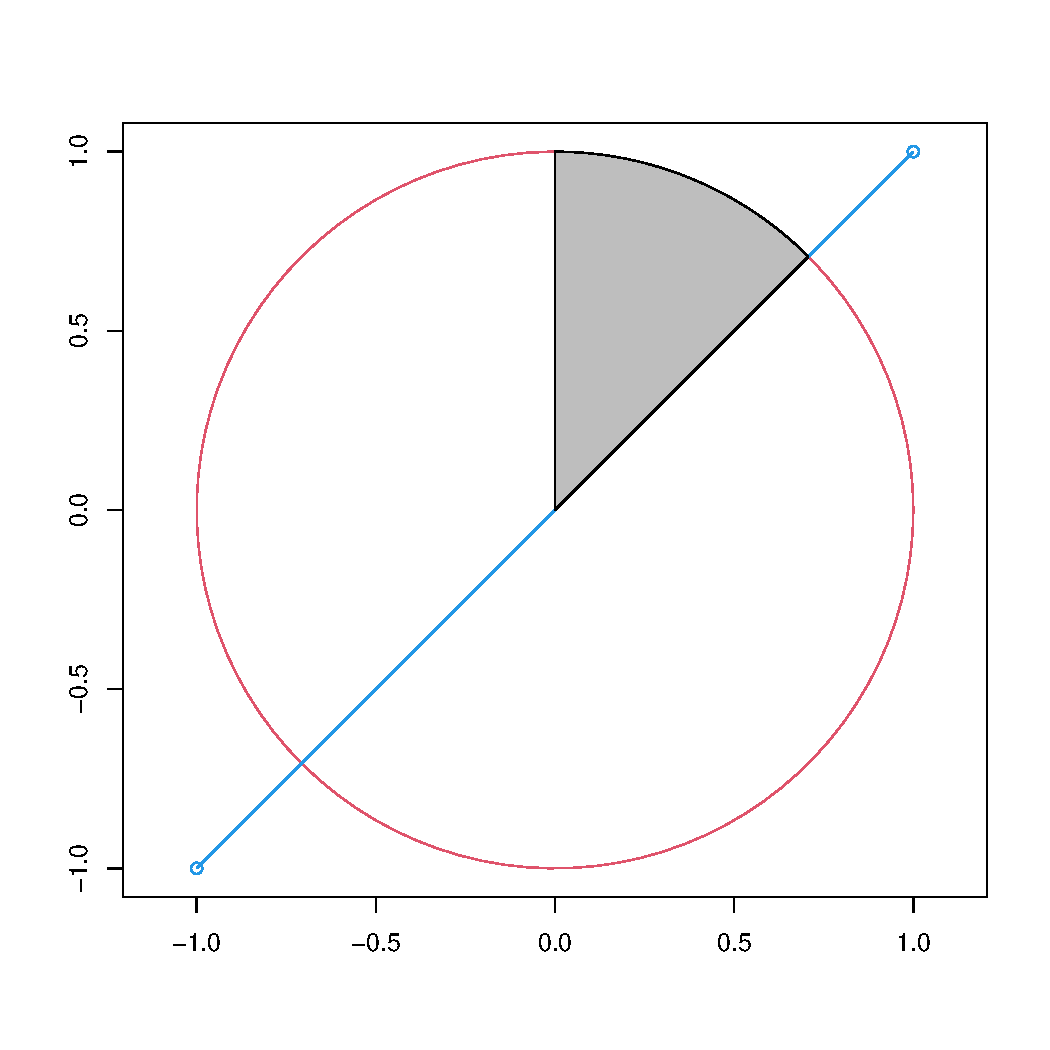
\includegraphics[width=200pt]{Domain_1_1_R.pdf}
%            \end{wrapfigure}
            \end{center}

            $y$を先に積分する場合、
            $y$の積分範囲は
            直線$y=x$上の点から円周上の点の区間となる。
            \begin{align}
             \iint_{D} (x^2-y^2) dxdy
               = 
             \int_{0}^{1/\sqrt{2}}
               \int_{x}^{\sqrt{1-x^2}}
                 (x^2-y^2)
               dy
             dx
%             \\
%             = &
%             \int_{0}^{1/\sqrt{2}}
%               \left[ x^2y-\frac{y^3}{3} \right]_{y=x}^{y=\sqrt{1-x^2}}
%             dx\\
%             = &
%             \int_{0}^{1/\sqrt{2}}
%               \left(
%                 \frac{\sqrt{1-x^2}}{3}(4x^2-1)
%                 -
%                 \frac{2}{3}x^3
%               \right)
%             dx\\
            \end{align}

            $x$を先に積分する場合は
            積分を分けて考える必要がある。

            極座標に変換する場合、
            $x=r\cos\theta,\ y=r\sin\theta$と置く。
            それぞれの積分範囲は$r:0\to1,\ \theta:\pi/4\to\pi/2$
            であり、
            ヤコビ行列式より
            $dxdy=rdrd\theta$である。

            \begin{equation}
              \iint_{D} (x^2-y^2) dxdy
               =
              \int_{0}^{1}
              \int_{\frac{\pi}{4}}^{\frac{\pi}{2}}
                (r^2\cos^2\theta - r^2\sin^2\theta)
              \cdot r d\theta dr
            \end{equation}

            $r^2\cos^2\theta - r^2\sin^2\theta = r^2\cos 2\theta$
            であるので、積分は次のように計算できる。

            \begin{align}
              \iint_{D} (x^2-y^2) dxdy
               =&
              \int_{0}^{1}
              \int_{\frac{\pi}{4}}^{\frac{\pi}{2}}
                r^2\cos2\theta
              \cdot r d\theta dr %\\
               = %&
              \int_{0}^{1} r^3 dr
              \int_{\frac{\pi}{4}}^{\frac{\pi}{2}} \cos 2\theta d\theta\\
             =&
             \left[ \frac{1}{4}r^4\right]_{r=0}^{r=1}
             \left[ \frac{1}{2}\sin 2\theta \right]_{\theta = \frac{\pi}{4}}^{\theta =\frac{\pi}{2}} %\\
             = %&
             \frac{1}{4} \cdot \left( -\frac{1}{2} \right)
             = - \frac{1}{8}
            \end{align}


            \hrulefill

       \item
            \begin{equation}
             \iiint_{E} \frac{x^2+y^2}{\sqrt{x^2+y^2+z^2}}dxdydz
              ,\quad
              E=\{
                (x,y,z) \mid x^2 + y^2 + z^2 \leq 1,\ z\geq 0
              \}
            \end{equation}

            \dotfill

            $E\subset \mathbb{R}^3$とする。

            領域$E$は$z \geq 0$の範囲で切り取られた半球である。

            次のように極座標変換を行う。
            \begin{equation}
              x = r \sin\theta \cos\varphi
              ,\quad
              y = r \sin\theta \sin\varphi
              ,\quad
              z = r\cos\theta
            \end{equation}

            $E$より$r,\theta,\varphi$の積分範囲は
            次のようになる。
            \begin{equation}
             0\leq r \leq 1
              ,\quad
              0 \leq \theta \leq \frac{\pi}{2}
              ,\quad
              0 \leq \varphi \leq 2\pi
            \end{equation}

            ヤコビアンを計算する。
            \begin{equation}
             \left\lvert
             \frac{\partial(x,y,z)}{\partial(r,\theta,\varphi)}
             \right\rvert
              =
              \begin{vmatrix}
               x_{r} & x_{\theta} & x_{\varphi} \\
               y_{r} & y_{\theta} & y_{\varphi} \\
               z_{r} & z_{\theta} & z_{\varphi}
              \end{vmatrix}
              = r^2\sin\theta
            \end{equation}

            これにより
            $dxdydz = r^2\sin\theta\ drd\theta d\varphi$
            となる。

            変数変換により
            $\sqrt{x^2+y^2+z^2}=r,\ x^2+y^2=r^2\sin^2\theta$
            であるので、
            問題の式は次のようになる。
            \begin{equation}
             \iiint_{E} \frac{x^2+y^2}{\sqrt{x^2+y^2+z^2}}dxdydz
              =
             \int_{0}^{1}
               \int_{0}^{\frac{\pi}{2}}
                 \int_{0}^{2\pi}
                 r\sin^2\theta \cdot r^2\sin\theta\
                 d\varphi
               d\theta
             dr
            \end{equation}

            3倍角の公式
            $\sin3\theta = 3\sin\theta -4 \sin^3\theta$
            を利用し計算を行う。
            \begin{align}
             &
             \int_{0}^{1}
               \int_{0}^{\frac{\pi}{2}}
                 \int_{0}^{2\pi}
                 r^3\sin^3\theta \
                 d\varphi
               d\theta
             dr\\
             =&
             \int_{0}^{1} r^3 dr
               \int_{0}^{\frac{\pi}{2}} \frac{3\sin\theta - \sin 3\theta}{4}
                 \int_{0}^{2\pi} d\varphi
             \\
             =&
               \left[ \frac{1}{4}r^4\right]_{r=0}^{r=1}
               \left[ -\frac{3}{4}\cos\theta + \frac{1}{12}\cos 3\theta \right]_{\theta=0}^{\theta=\frac{\pi}{2}}
               \left[ \varphi \right]_{\varphi=0}^{\varphi=2\pi}
             \\
             =&
             \frac{1}{4}
             \cdot \left( \frac{3}{4} - \frac{1}{12} \right)
             \cdot 2\pi
             = \frac{\pi}{3}
            \end{align}


            \hrulefill

      \end{enumerate}
      \hrulefill
 \item
      次の積分の順序を交換せよ。
      ただし、$f$は積分の順序を交換できる関数とする。

      \begin{enumerate}
       \item
            \begin{equation}
             \int_{-1}^{0}dx\int_{0}^{1+x} f(x,y)dy
              + \int_{0}^{1}dx\int_{0}^{1-x} f(x,y)dy
            \end{equation}

            \dotfill

            \includegraphics[width=200pt]{int_2_1.pdf}

            1つ目の積分範囲は
            $-1 \leq x \leq 0,\ 0 \leq y \leq 1+x$
            であり、
            2つ目の積分範囲は
            $0 \leq x \leq 1,\ 0 \leq y \leq 1-x$
            である。
            図では1つ目の積分領域が緑、2つ目は青である。

            問いの積分は
            $y$について積分してから
            $x$について積分をする。
            縦向けの積分なので、
            $y=0$から$y=1+x$または$y=1-x$までの積分となるため
            2つに分けている。
            先に横向けの積分を行えば一つにまとめることができる。

            $x$は$y=1+x$から$y=1-x$まで区間で積分をして、
            そのあと、$y$は$0$から$1$に積分をする。

            \begin{align}
             \int_{-1}^{0}dx\int_{0}^{1+x} f(x,y)dy
              +& \int_{0}^{1}dx\int_{0}^{1-x} f(x,y)dy\\
              &=
             \int_{0}^{1} \int_{y-1}^{-y+1} f(x,y) dxdy
            \end{align}

            \hrulefill

       \item
            \begin{equation}
             \int_{-1}^{0}dy\int_{0}^{1+\sqrt{1-(y+1)^2}} f(x,y)dx
              + \int_{0}^{1}dy\int_{0}^{1-\sqrt{1-(y-1)^2}} f(x,y)dx
            \end{equation}

            \dotfill

            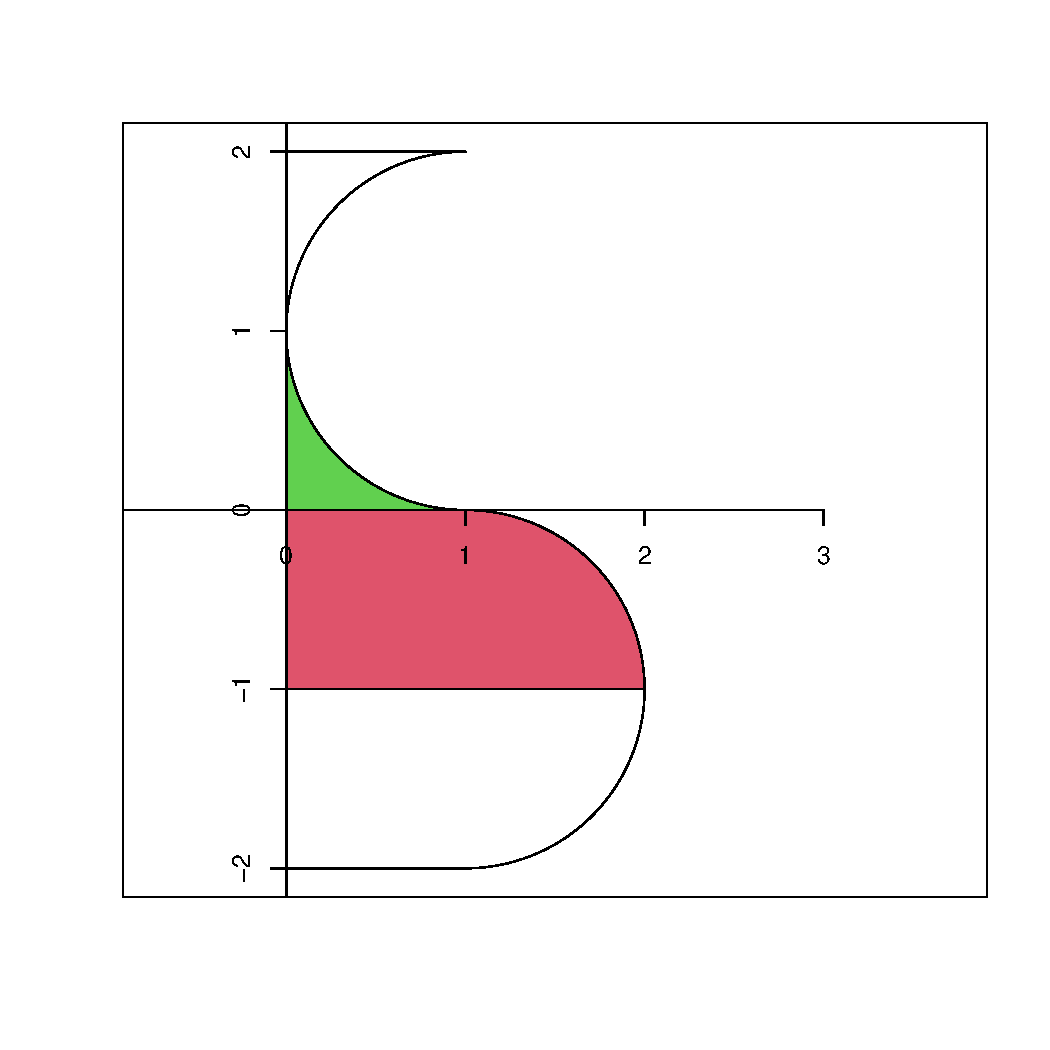
\includegraphics[width=200pt]{int_2_2_1a.pdf}

            1つ目の積分範囲は
            $-1\leq y \leq 0,\ 0\leq x \leq 1+\sqrt{1-(y+1)^2}$
            である。
            $0\leq x \leq 1+\sqrt{1-(y+1)^2}$は
            中心$(1,-1)$で半径1の円の右半分から
            $y$軸までの領域を指しており、
            $-1\leq y \leq 0$で範囲を制限したものが、
            上の図の下側の図形(赤)である。

            2つ目の積分範囲は
            $0\leq y \leq 1,\ 0\leq x \leq 1-\sqrt{1-(y-1)^2}$
            である。
            $0\leq x \leq 1-\sqrt{1-(y-1)^2}$
            は
            中心$(1,1)$で半径1の円の左半分から
            $y$軸までの領域を指しており、
            $0\leq y \leq 1$に制限したものが、
            上の図の上側の図形(緑)である。

            変数$y$について先に積分した後、
            $x$について積分を行うので、
            $0\leq x \leq 1$と$1\leq x \leq 2$
            の二つに分けて考える。

            $0\leq x \leq 1$の範囲では
            $-2\leq y \leq 1-\sqrt{1-(x-1)^2}$
            であるので、
            積分は次の式で表せる。
            \begin{equation}
             \int_{0}^{1} \int_{-2}^{1-\sqrt{1-(x-1)^2}} f(x,y) dy dx
            \end{equation}

            $1\leq x \leq 2$の範囲では
            $-2\leq y \leq -1+\sqrt{1-(x-1)^2}$
            であるので、
            積分は次の式で表せる。
            \begin{equation}
             \int_{1}^{2} \int_{-2}^{-1+\sqrt{1-(x-1)^2}} f(x,y) dy dx
            \end{equation}


            よって、積分順を入れ替えると次のようになる。
            \begin{align}
             & \int_{-1}^{0}dy\int_{0}^{1+\sqrt{1-(y+1)^2}} f(x,y)dx
              + \int_{0}^{1}dy\int_{0}^{1-\sqrt{1-(y-1)^2}} f(x,y)dx\\
%             =&
%             \int_{0}^{1} \int_{-2}^{1-\sqrt{1-(x-1)^2}} f(x,y) dy dx
%             +
%             \int_{1}^{2} \int_{-2}^{-1+\sqrt{1-(x-1)^2}} f(x,y) dy dx\\
             =&
             \int_{0}^{1} dx \int_{-2}^{1-\sqrt{1-(x-1)^2}} f(x,y) dy
             +
             \int_{1}^{2} dx \int_{-2}^{-1+\sqrt{1-(x-1)^2}} f(x,y) dy
            \end{align}


            \hrulefill

      \end{enumerate}
\end{enumerate}


\hrulefill

\end{document}
